% Asset ID: FA22CentreOfMassTikZ-003
% Source: Phase 4 generated TikZ asset for FA22 Centre of Mass
% Related lesson section: Section 9 TikZ placeholders
% Purpose: Composite lamina grid.
\documentclass[tikz,border=8pt]{standalone}
\usepackage{amsmath}
\definecolor{Canvas}{HTML}{FAF9F6}
\definecolor{Ink}{HTML}{2C2C2E}
\definecolor{LineSoft}{HTML}{E5E5EA}
\definecolor{Gold}{HTML}{D4AF37}
\definecolor{Accent}{HTML}{C5A059}
\definecolor{Blush}{HTML}{FBEFEF}
\begin{document}
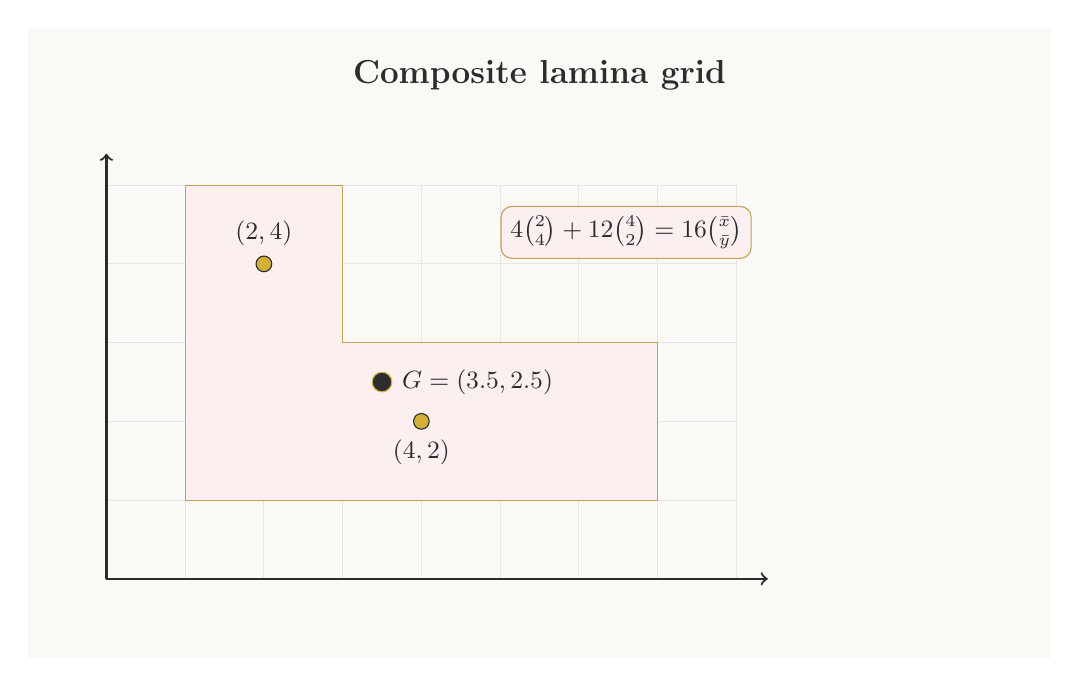
\begin{tikzpicture}[every node/.style={font=\small,text=Ink},line/.style={draw=Ink,line width=0.8pt},gold/.style={draw=Accent,line width=1.1pt},dot/.style={circle,fill=Gold,draw=Ink,inner sep=2pt}]
\fill[Canvas] (-1,-1) rectangle (12,7);
\node[font=\bfseries\large] at (5.5,6.4) {Composite lamina grid};

\draw[step=1,draw=LineSoft] (0,0) grid (8,5);\draw[line,->] (0,0)--(8.4,0);\draw[line,->] (0,0)--(0,5.4);
\draw[fill=Blush,draw=Accent] (1,1)--(7,1)--(7,3)--(3,3)--(3,5)--(1,5)--cycle;
\node[dot,label=above:{$(2,4)$}] at (2,4){};\node[dot,label=below:{$(4,2)$}] at (4,2){};\node[circle,fill=Ink,draw=Gold,inner sep=2.5pt,label=right:{$G=(3.5,2.5)$}] at (3.5,2.5){};
\node[draw=Accent,fill=Blush,rounded corners,align=center] at (6.6,4.4){$4\binom24+12\binom42=16\binom{\bar{x}}{\bar{y}}$};
\end{tikzpicture}
\end{document}
